%%%%%%%%%%%%%%%%%%%%%%%%%%%%%%%%%%%%%%%%%
% NIWeek 2014 Poster by T. Reveyrand
% www.microwave.fr
% http://www.microwave.fr/LaTeX.html
% ---------------------------------------
% 
% Original template created by:
% Brian Amberg (baposter@brian-amberg.de)
%
% This template has been downloaded from:
% http://www.LaTeXTemplates.com
%
% License:
% CC BY-NC-SA 3.0 (http://creativecommons.org/licenses/by-nc-sa/3.0/)
%
%%%%%%%%%%%%%%%%%%%%%%%%%%%%%%%%%%%%%%%%%

%----------------------------------------------------------------------------------------
%	PACKAGES AND OTHER DOCUMENT CONFIGURATIONS
%----------------------------------------------------------------------------------------

\documentclass[a0paper,portrait]{baposter}
\usepackage[font=small,labelfont=bf]{caption} % Required for specifying captions to tables and figures
\usepackage{booktabs} % Horizontal rules in tables
\usepackage{relsize} % Used for making text smaller in some places
\usepackage{natbib} \bibpunct{(}{)}{;}{author-year}{}{,}
\bibliographystyle{genetics}
\usepackage{amsmath,amsfonts,amssymb,amsthm} % Math packages
\usepackage{eqparbox}

\usepackage{textcomp}
\usepackage{multicol}
\usepackage{wrapfig} % Allows wrapping text around tables and figures

\graphicspath{{figures/}} % Directory in which figures are stored

 %\definecolor{bordercol}{RGB}{40,40,40} % Border color of content boxes
 \definecolor{bordercol}{rgb}{1.0, 0.55, 0.0}
 \definecolor{headercol1} {RGB}{186,215,230} % Background color for the header in the content boxes (left side)
 \definecolor{headercol2}{RGB}{120,120,120} % Background color for the header in the content boxes (right side)
 \definecolor{headerfontcol}{rgb}{0,0,0} % Text color for the header text in the content boxes
 \definecolor{boxcolor}{RGB}{210,235,250} % Background color for the content in the content boxes


\begin{document}

\background{ % Set the background to an image (background.pdf)
\begin{tikzpicture}[remember picture,overlay]
\draw (current page.north west)+(-1em,1em) node[anchor=north west]
{\includegraphics[height=1.1\textheight]{background}};
\end{tikzpicture}
}

\begin{poster}{
grid=false,
borderColor=bordercol, % Border color of content boxes
headerColorOne=headercol1, % Background color for the header in the content boxes (left side)
headerColorTwo=headercol2, % Background color for the header in the content boxes (right side)
headerFontColor=headerfontcol, % Text color for the header text in the content boxes
boxColorOne=boxcolor, % Background color for the content in the content boxes
headershape=roundedright, % Specify the rounded corner in the content box headers
headerfont=\Large\sf\bf, % Font modifiers for the text in the content box headers
textborder=rectangle,
background=user,
headerborder=open, % Change to closed for a line under the content box headers
boxshade=plain
}
{
\includegraphics[scale=0.07]{Clemson_logo.png}}
%
%----------------------------------------------------------------------------------------
%	TITLE AND AUTHOR NAME
%----------------------------------------------------------------------------------------
%
{\bf  \huge {Genome-Wide Prediction, Association, and Gene Network Analysis of Grain Composition in Sorghum} }
%\Large \it A} % Poster title
{\large \textbf{Sirjan Sapkota}$^{1,2,*}$, J. Lucas Boatwright$^{1,2}$, Richard Boyles$^{2,3}$, and Stephen Kresovich$^{1,2}$\\  % Author names
 
\small $^1$\it {Advanced Plant Technology Program, Clemson University, Clemson, SC 29634}\\ % Author addresses
\small $^2$\it {Department of Plant and Environmental Sciences, Clemson University, Clemson, SC 29634}\\ % Author addresses
\small $^3$\it {Pee Dee Research and Education Center, Clemson University, Darlington, SC 29532}\\ % Author addresses
\small $^*$\it {Correspondence: \textbf{ssapkot@clemson.edu}; GitHub: sirjansapkota; LinkedIn: sirjan-sapkota-09787049}
} % Author contact
{
\includegraphics[scale=0.25]{figures/TigerPaw_co.png}}% University/lab logo
\vspace{-2 cm}
%----------------------------------------------------------------------------------------
%	ABSTRACT
%----------------------------------------------------------------------------------------
\headerbox{Abstract}{name=abstract,column=0,row=0, span=3}{
\small{Starch and protein are two of the most important constituents of grain contributing to most of human and animal caloric needs. The genetic control of starch and protein composition are complex and not completely understood. While genome-wide prediction has been routinely studied for grain yield, little is done in terms of application of predictions for grain composition. Here we present our genotype-phenotype association and prediction study for starch, protein and gross energy using 224,007 SNPs in a sorghum diversity panel with 389 individuals. We did not find any significant difference in predictive ability between various Bayesian models with different priors. On average, the predictive ability was 0.6 for starch, 0.45 for protein, and 0.58 for gross energy. Using a multivariate linear mixed model for starch and protein, we were able to identify significant associations at genomic regions in chromosomes four and eight that were not significant using a univariate model for starch or protein alone. A total of 13 genes within linkage disequilibrium of the associated regions had high confidence (0.7) first interactors using STRING. The gene network analysis of those 13 genes and their first interactors showed significant enrichment for various biochemical pathways including sucrose and starch biosynthesis and nitrogen metabolism. Our results provide new insights into the application of multivariate approaches in statistical learning. Furthermore, the genes and pathways identified could be crucial in understanding genetic mechanisms in source-sink dynamics during grain filling.}
}
%----------------------------------------------------------------------------------------
%	Prediction
%----------------------------------------------------------------------------------------
\headerbox{Genomic Prediction}{name=prediction,column=1,row=1,span=1,below=abstract}
{
%\begin{wrapfigure}{l}{60mm}
\begin{center}
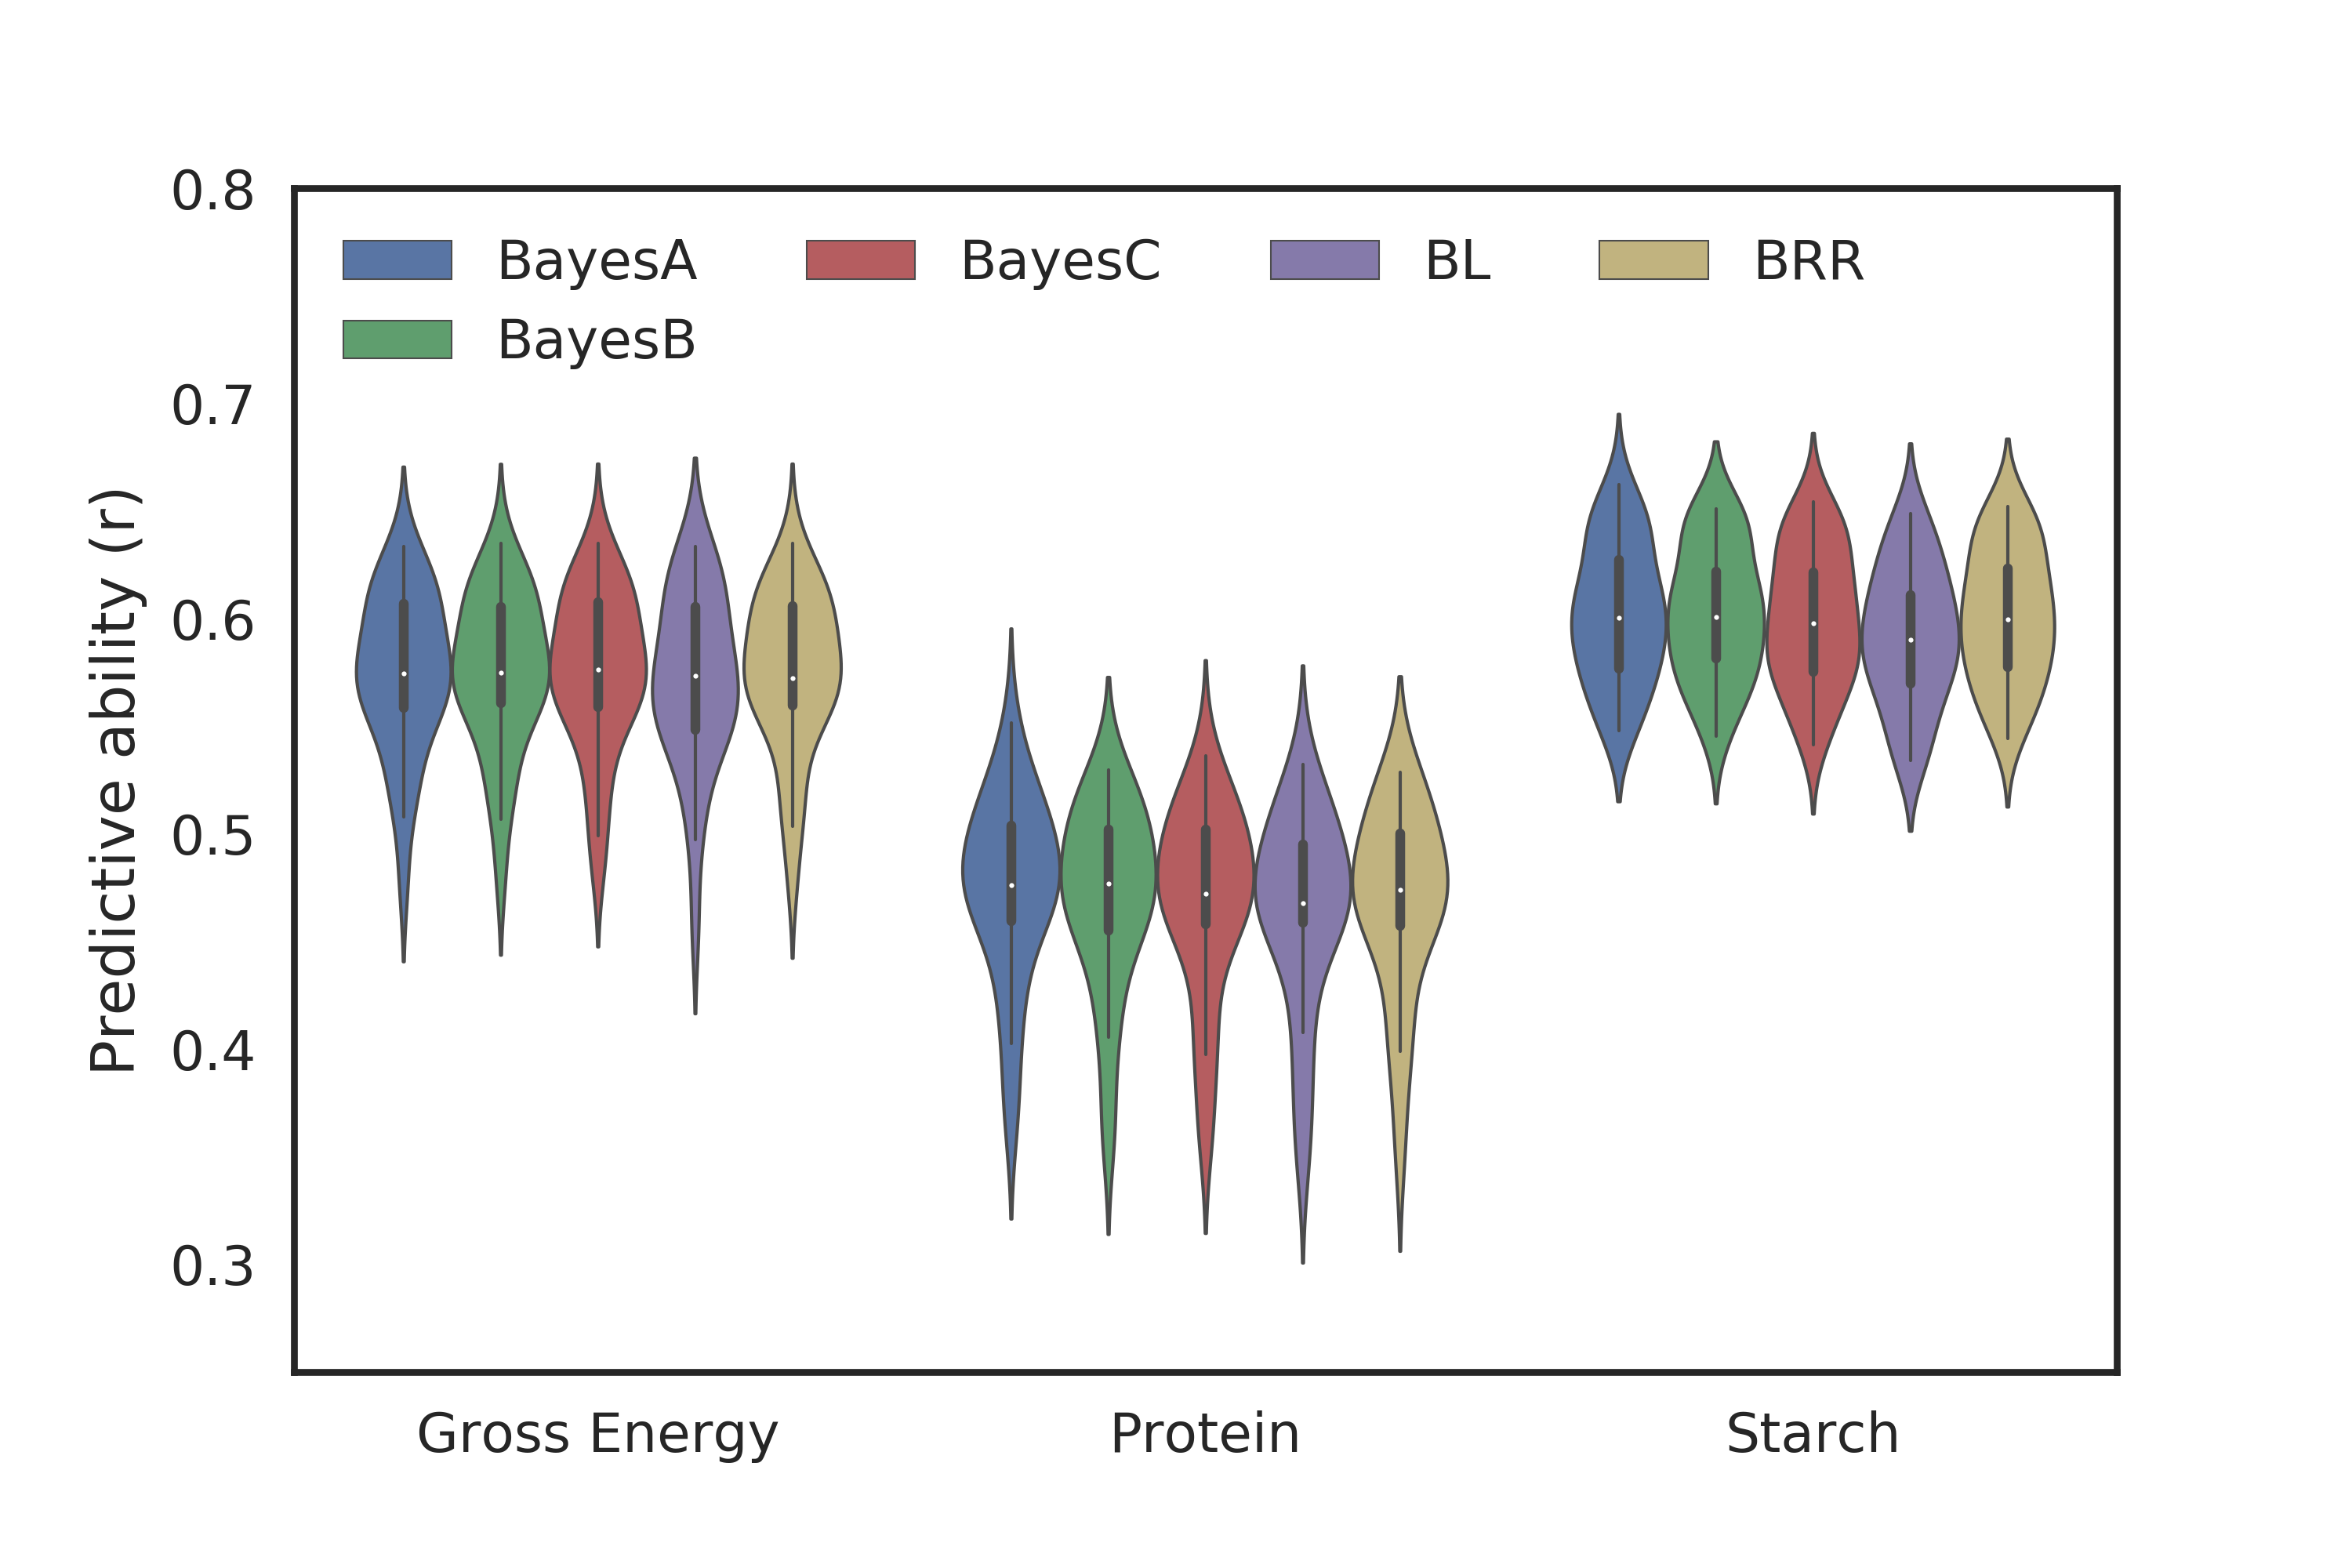
\includegraphics [height=45mm, width=70mm] {r_SAP-SPG_Models.png}
\end{center}
\textbf{Figure 3.} Results from five-fold cross validation of Bayesian whole genome regression using R package \textit{BGLR}. BRR: Bayesian ridge regression, BL: Bayesian lasso.
%\end{wrapfigure}
% \small{The KuPol instrument is a dual-beam receiver for the 40m telescope at OVRO. It is, in fact, a hybrid of two separate instruments called the analog and the digital instrument. The \textbf{Analog Instrument} is a dual-polarization, beam-differencing radiometer that is designed to produce identical data to the previous Ku-band, instrument that KuPol replaces. It is composed by the Cryostat, the Cold Plate, and UBE. The \textbf{Digital Instrument} is a digital spectropolarimeter that processes the band between 13 to 18 GHz in 500 MHz wide chunks with ∼8 MHz resolution. In this instrument is performed the signal distribution, downconversion, digitization and processing, and data readout and archiving.}
}
%----------------------------------------------------------------------------------------
%	Association
%----------------------------------------------------------------------------------------
\headerbox{Association Mapping}{name=association,column=2,row=1,span=1,below=abstract}
{
%\begin{wrapfigure}{l}{60mm}
\begin{center}
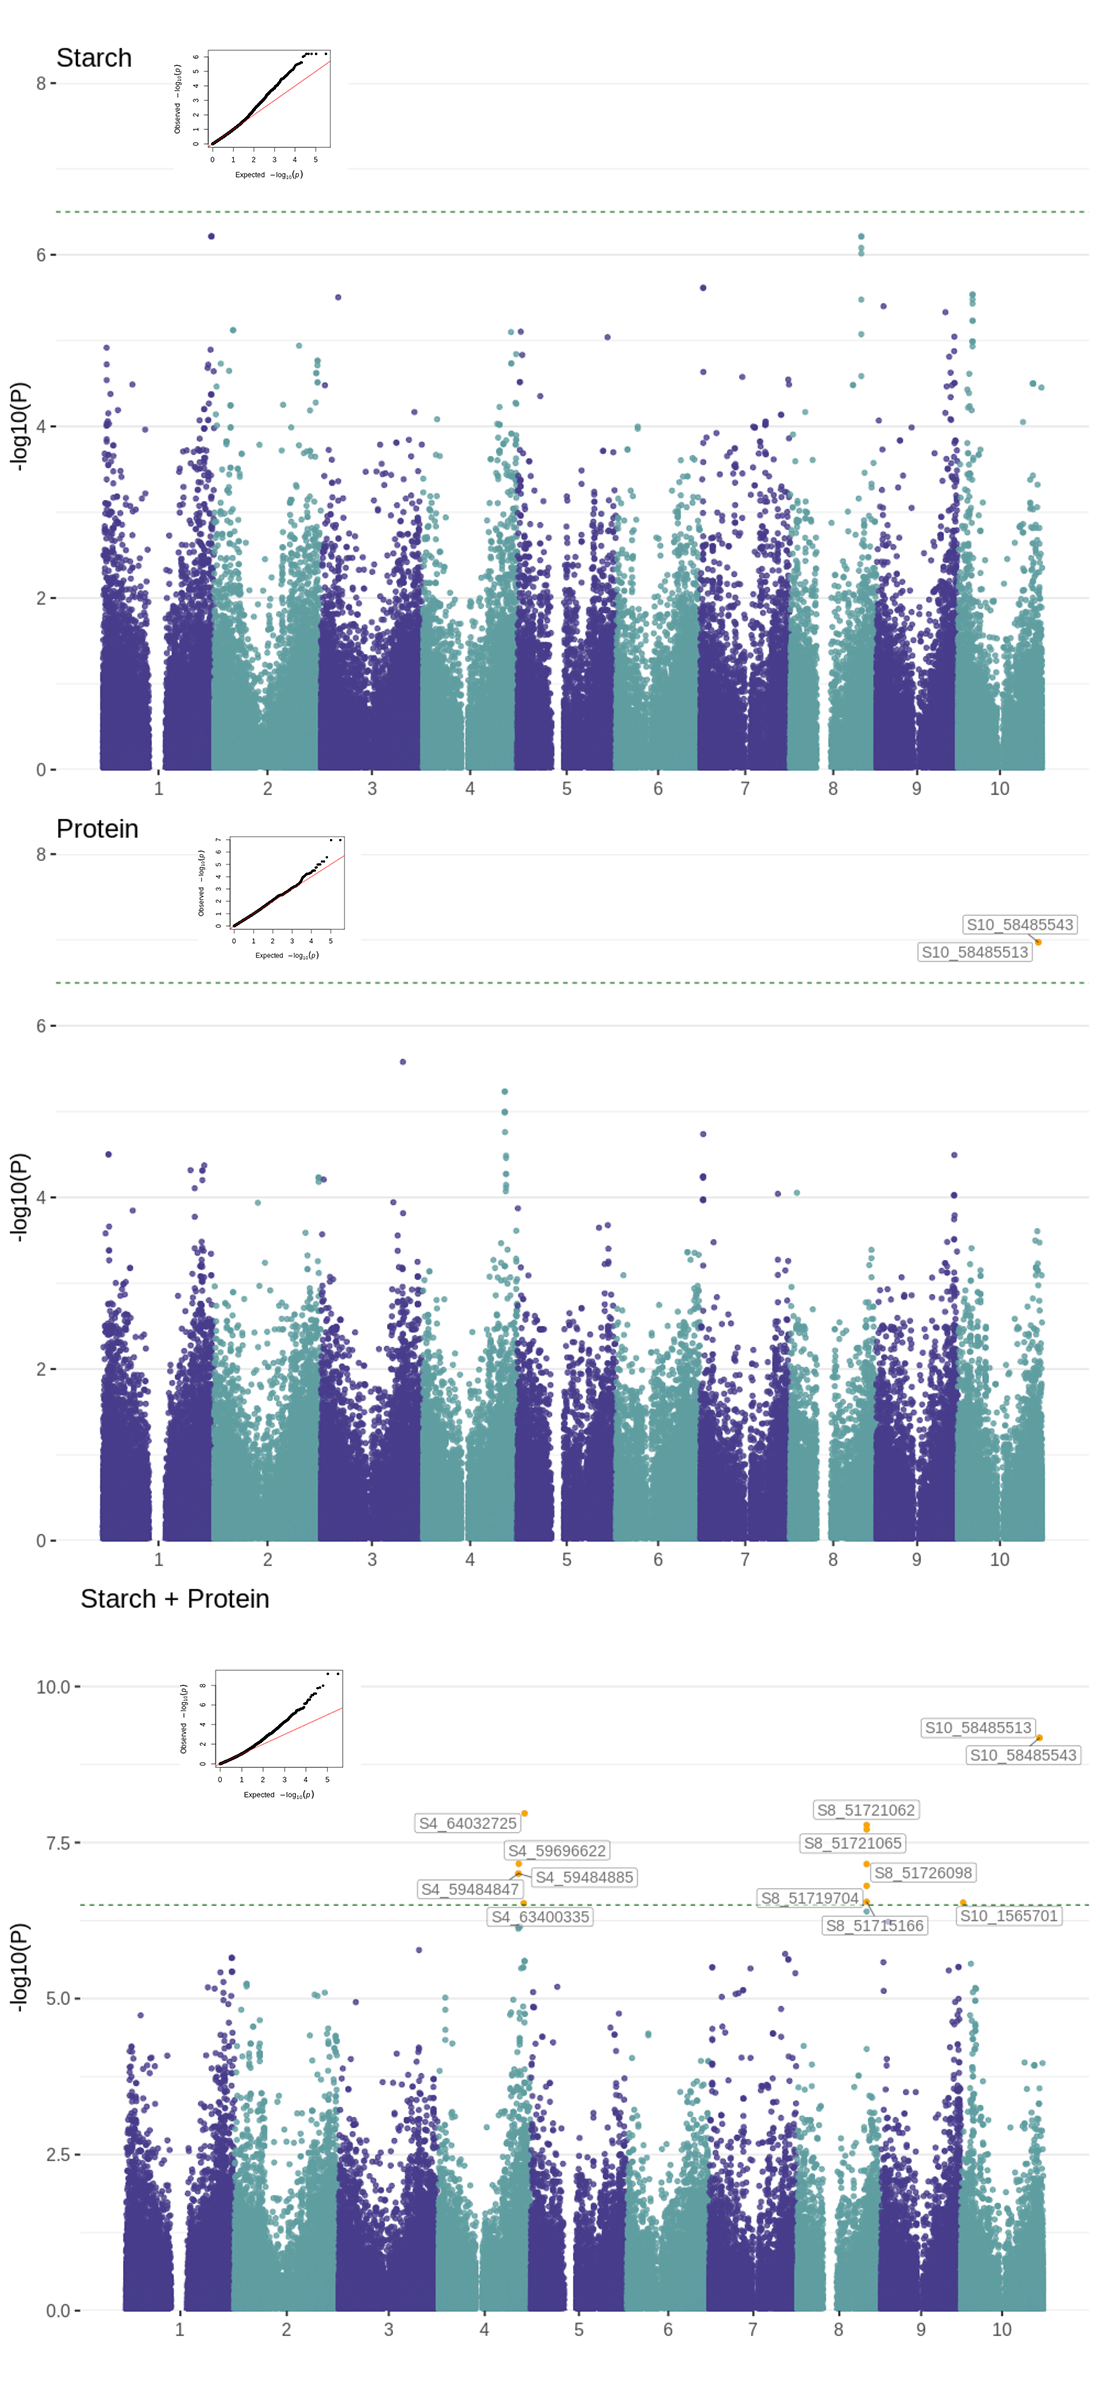
\includegraphics [height=120mm, width=70mm] {Starch_protein_GWAS_plots.png}
\end{center}
\textbf{Figure 4.} Manhattan plots for univariate (top 2) and multivariate (bottom) mixed model association analysis of starch and protein using software \textit{GEMMA}. Bonferroni significance threshold is shown by green dashed line.\\
}
%----------------------------------------------------------------------------------------
%	GENE NETWORK
%----------------------------------------------------------------------------------------
\headerbox{Gene Network}{name=genenetwork,column=1,row=1,span=1,below=prediction}
{
%\begin{wrapfigure}{l}{60mm}
\begin{center}
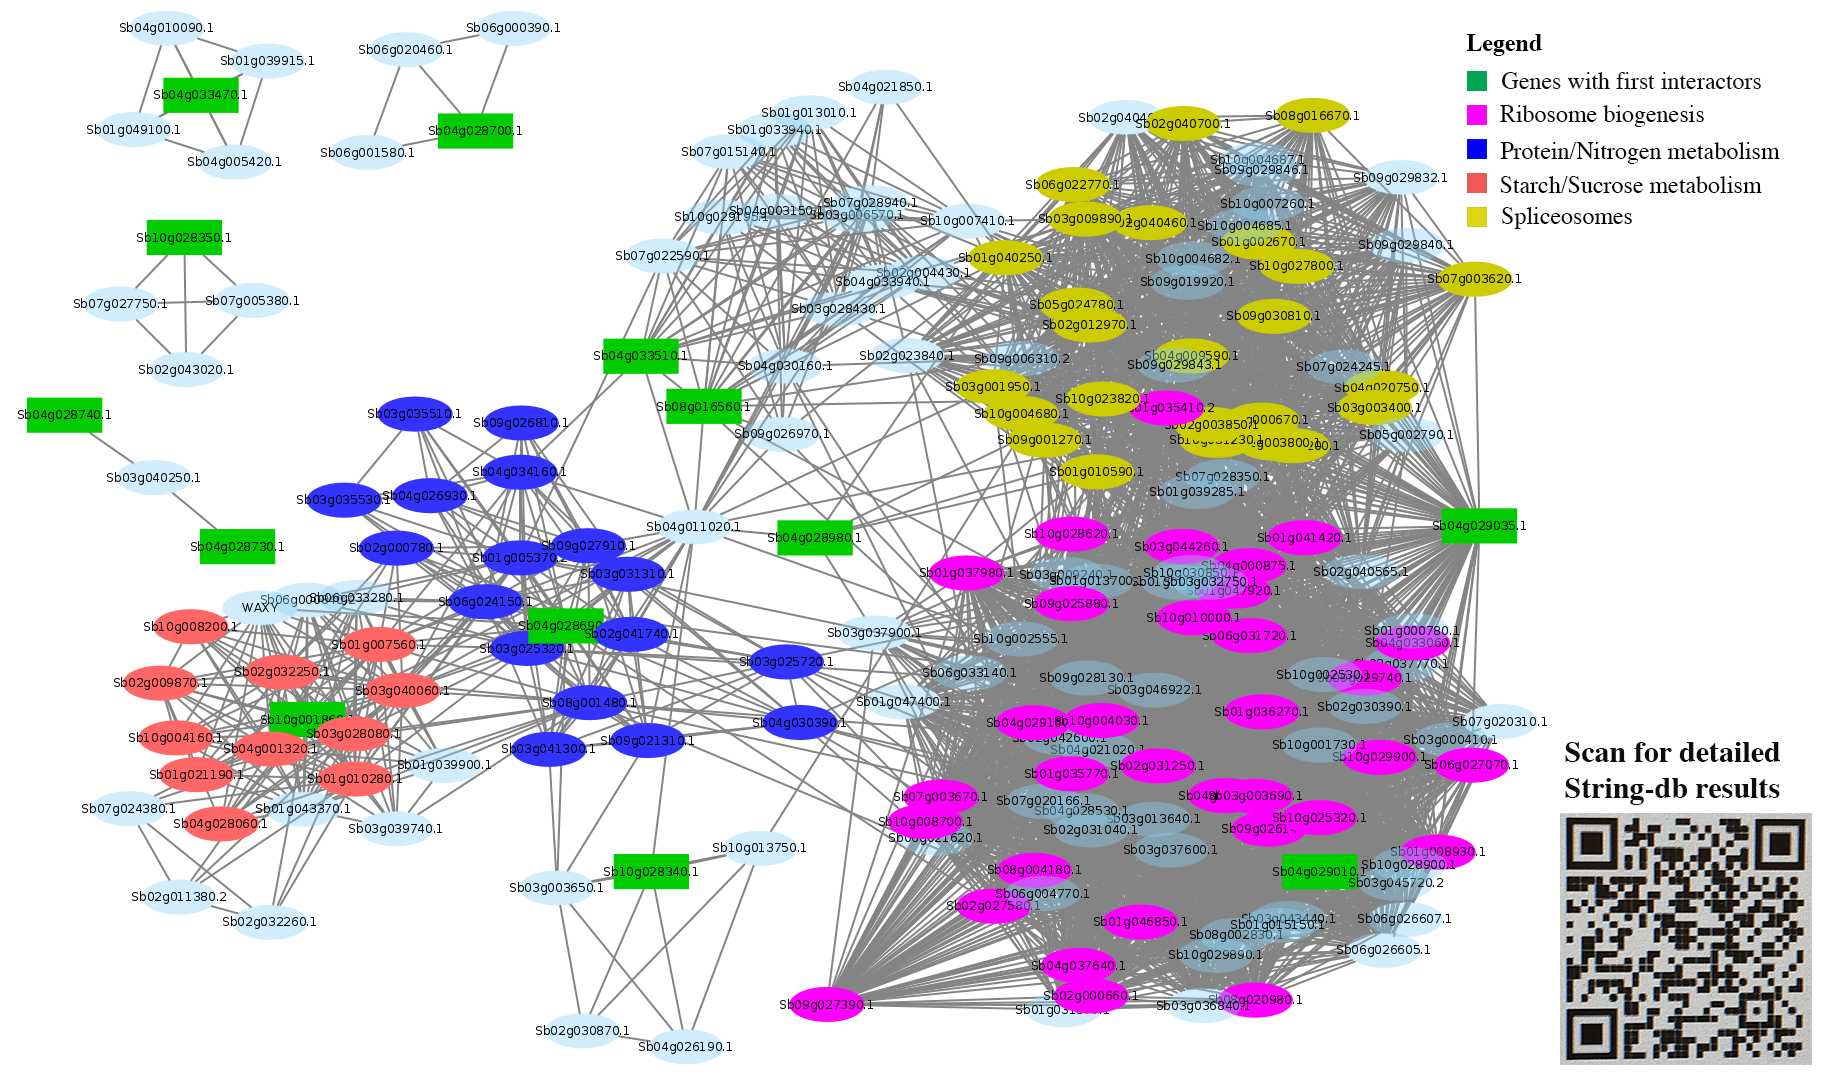
\includegraphics [height=44mm, width=70mm] {string_edited.png}
\end{center}
\textbf{Figure 5}. Gene network analysis for genes near significantly associated regions using \textit{STRING}. Among the genes within 20 kb of significant SNPs, we identified 13 (green) with high confidence first interactors (0.7) in STRING.}\\

%----------------------------------------------------------------------------------------
%	DATA
%----------------------------------------------------------------------------------------
\headerbox{Genotype and Phenotype}{name=genopheno, column=0,row=1,below=abstract}
{
\smaller{A total of 389 genetically diverse sorghum accessions, mostly from the sorghum association panel, were characterized with 224,007 SNP markers using genotyping-by-sequencing.}
\vspace{-0.5cm}
\begin{center}
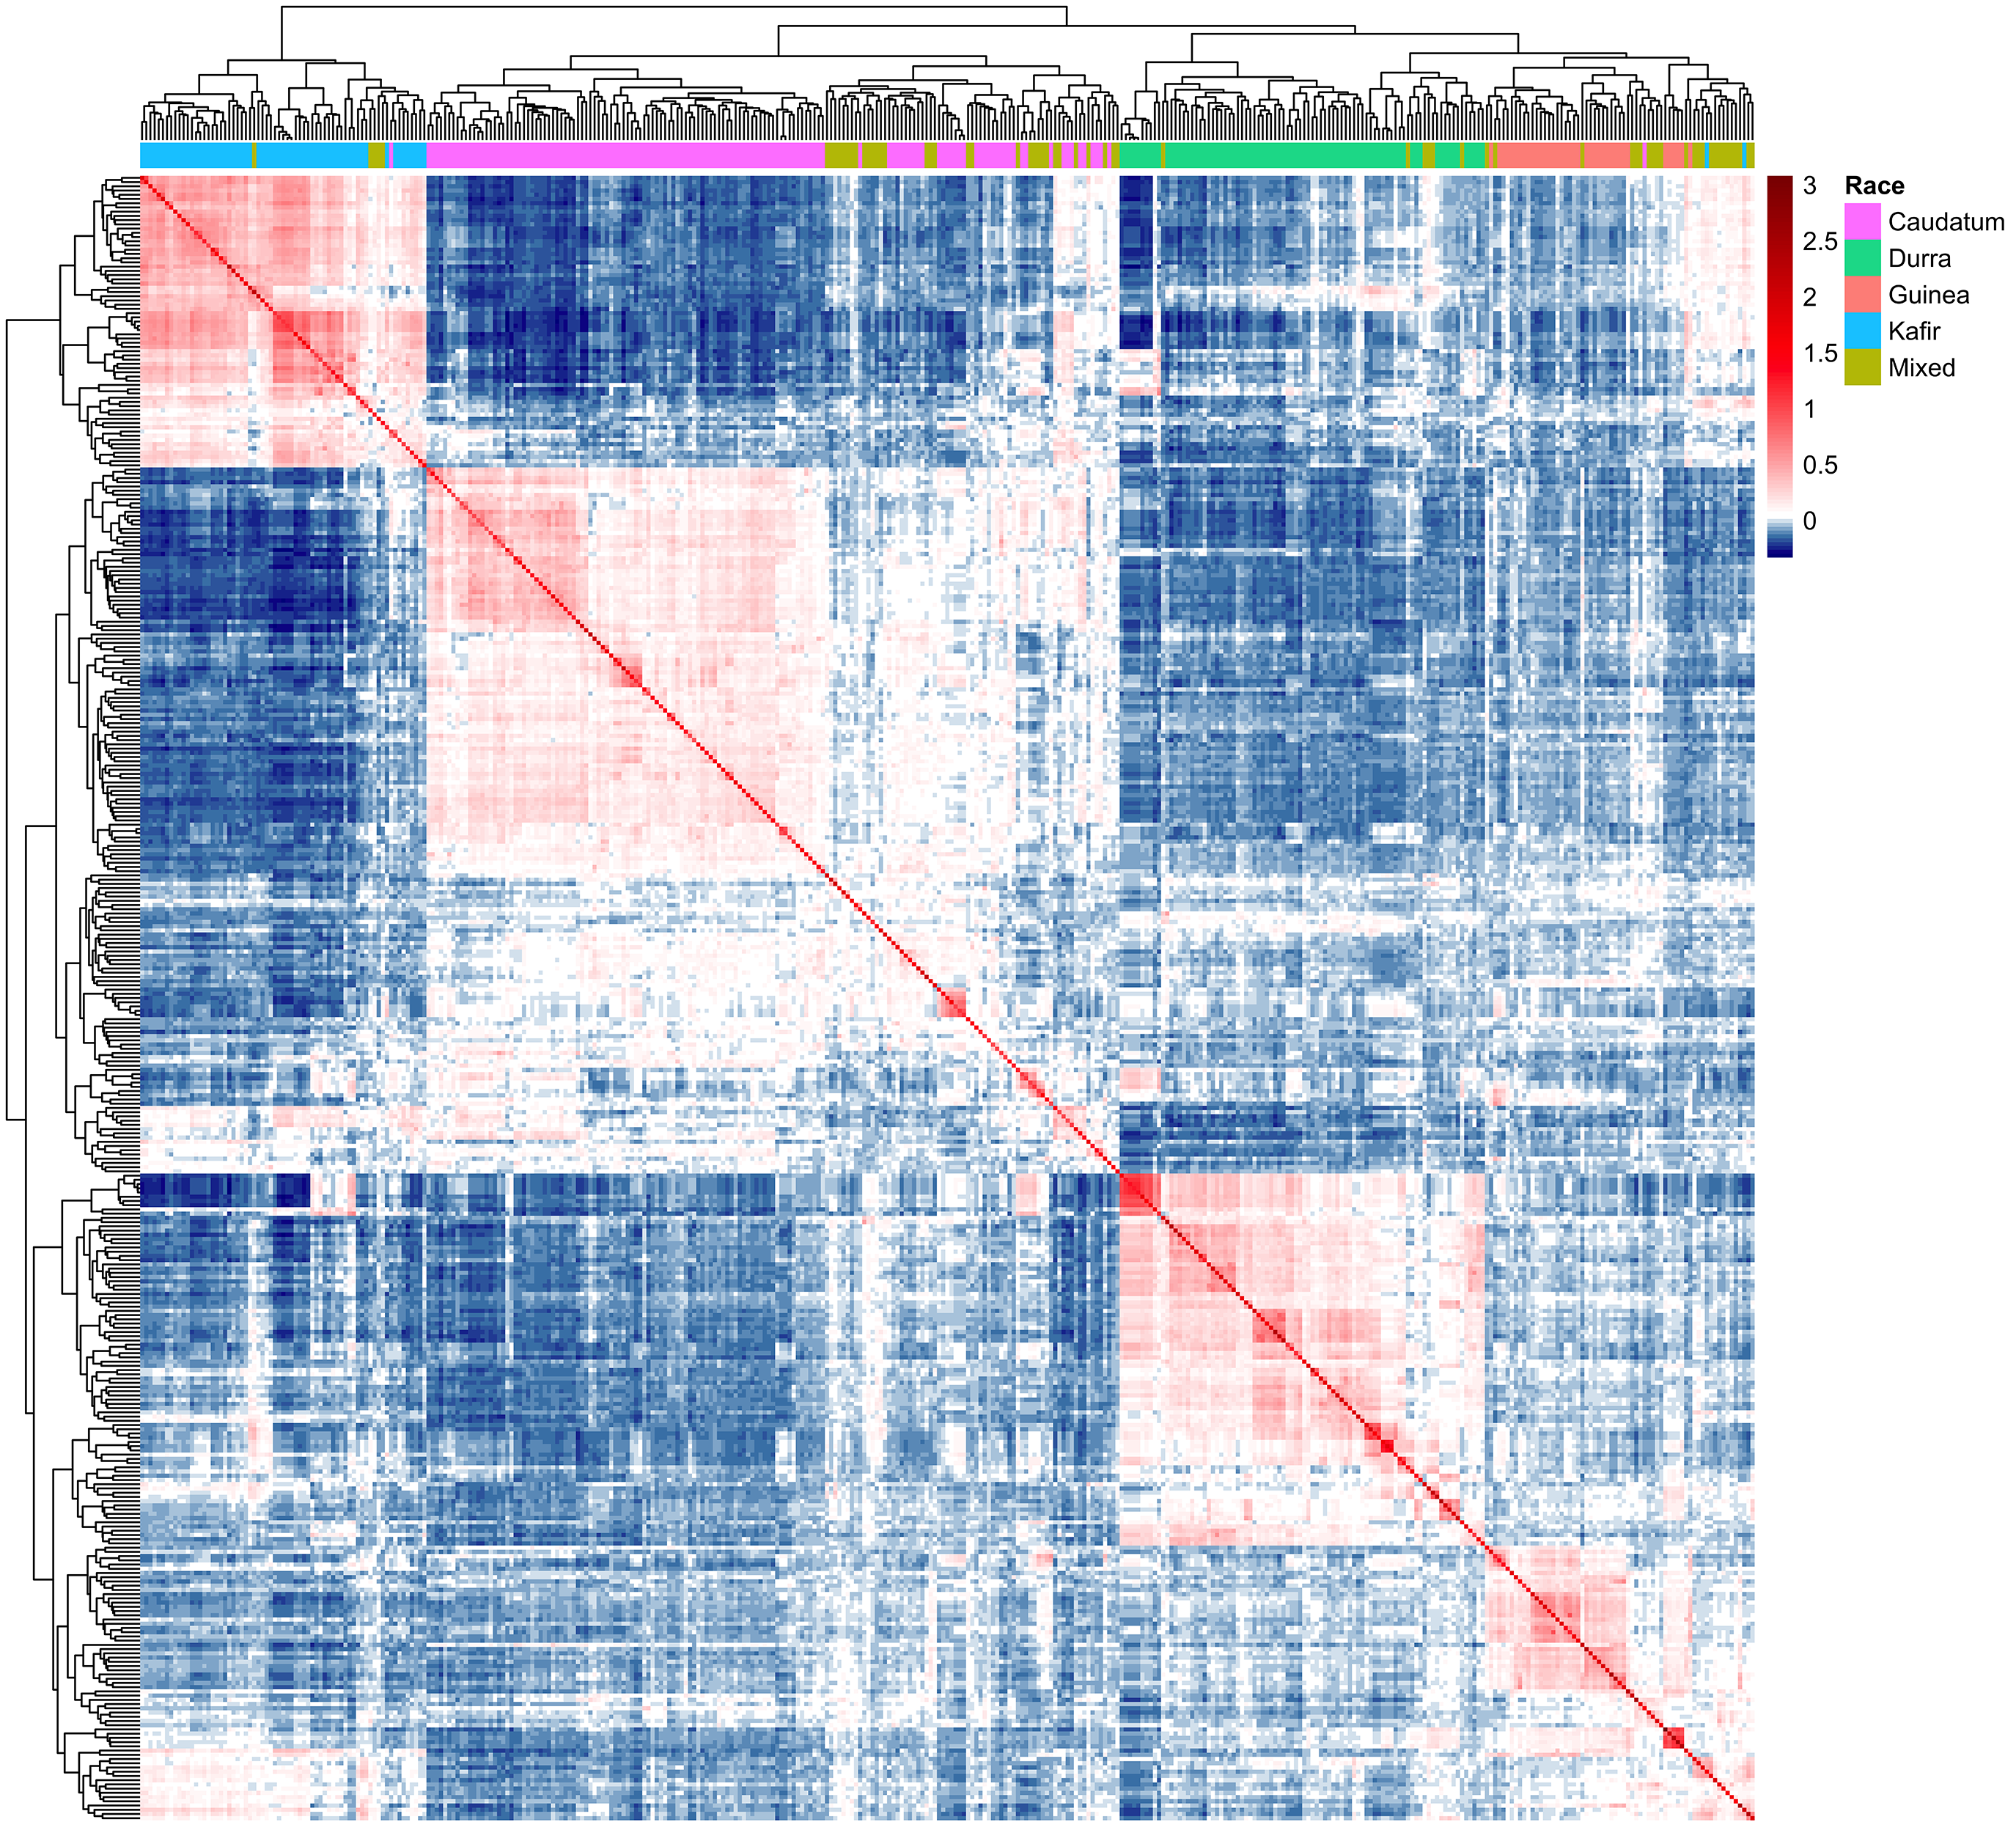
\includegraphics [height=65mm, width=74mm] {GRM_matrix.png}
\end{center}
\small{\textbf{Figure 1.} Heatmap of genomic relationship matrix computed using VanRaden(2008) method. Rug plot on top shows the racial classification of each genotype based on population structure analysis using \textit{ADMIXTURE} (K=5).}\\\\
\smaller {Grain of three random plants grown at Clemson Pee Dee Research and Education Center in Florence, SC during 2013, 2014, and 2017 were harvested at physiological maturity, ground and analyzed using near infrared spectroscopy (NIRS). Phenotypic best linear unbiased prediction (BLUPs) for each genotype (G) was calculated by adjusting phenotypic values (y) for random effects of year (Y), genotype-by-year (G $\times$ Y), and year-by-replication (Y $\times$ R) using a linear mixed model (1) in R package \textit{lme4}.
\begin{equation}
y \sim G + Y  +  G \times Y + Y \times R + \epsilon
\label{eqn:GSDP}
\end{equation}
% where $y_{ijk}$ represents the phenotypic values; $G_i$, $Y_j$, $E_l$, $G_i \times Y_j$, $G_i \times E_l$, $Y_j \times R_k$, $Y_i \times E_l \times R_k$ represent random effects of genotype, year, location, genotype-by-year, genotype-by-environment, replication-by-year, and replication-by-year-by-location respectively; and $\epsilon_{ijk}$/$\epsilon_{ijkl}$ is the random effect of residuals, with $N(0, \sigma_{\epsilon}^2)$.
}
\begin{center}
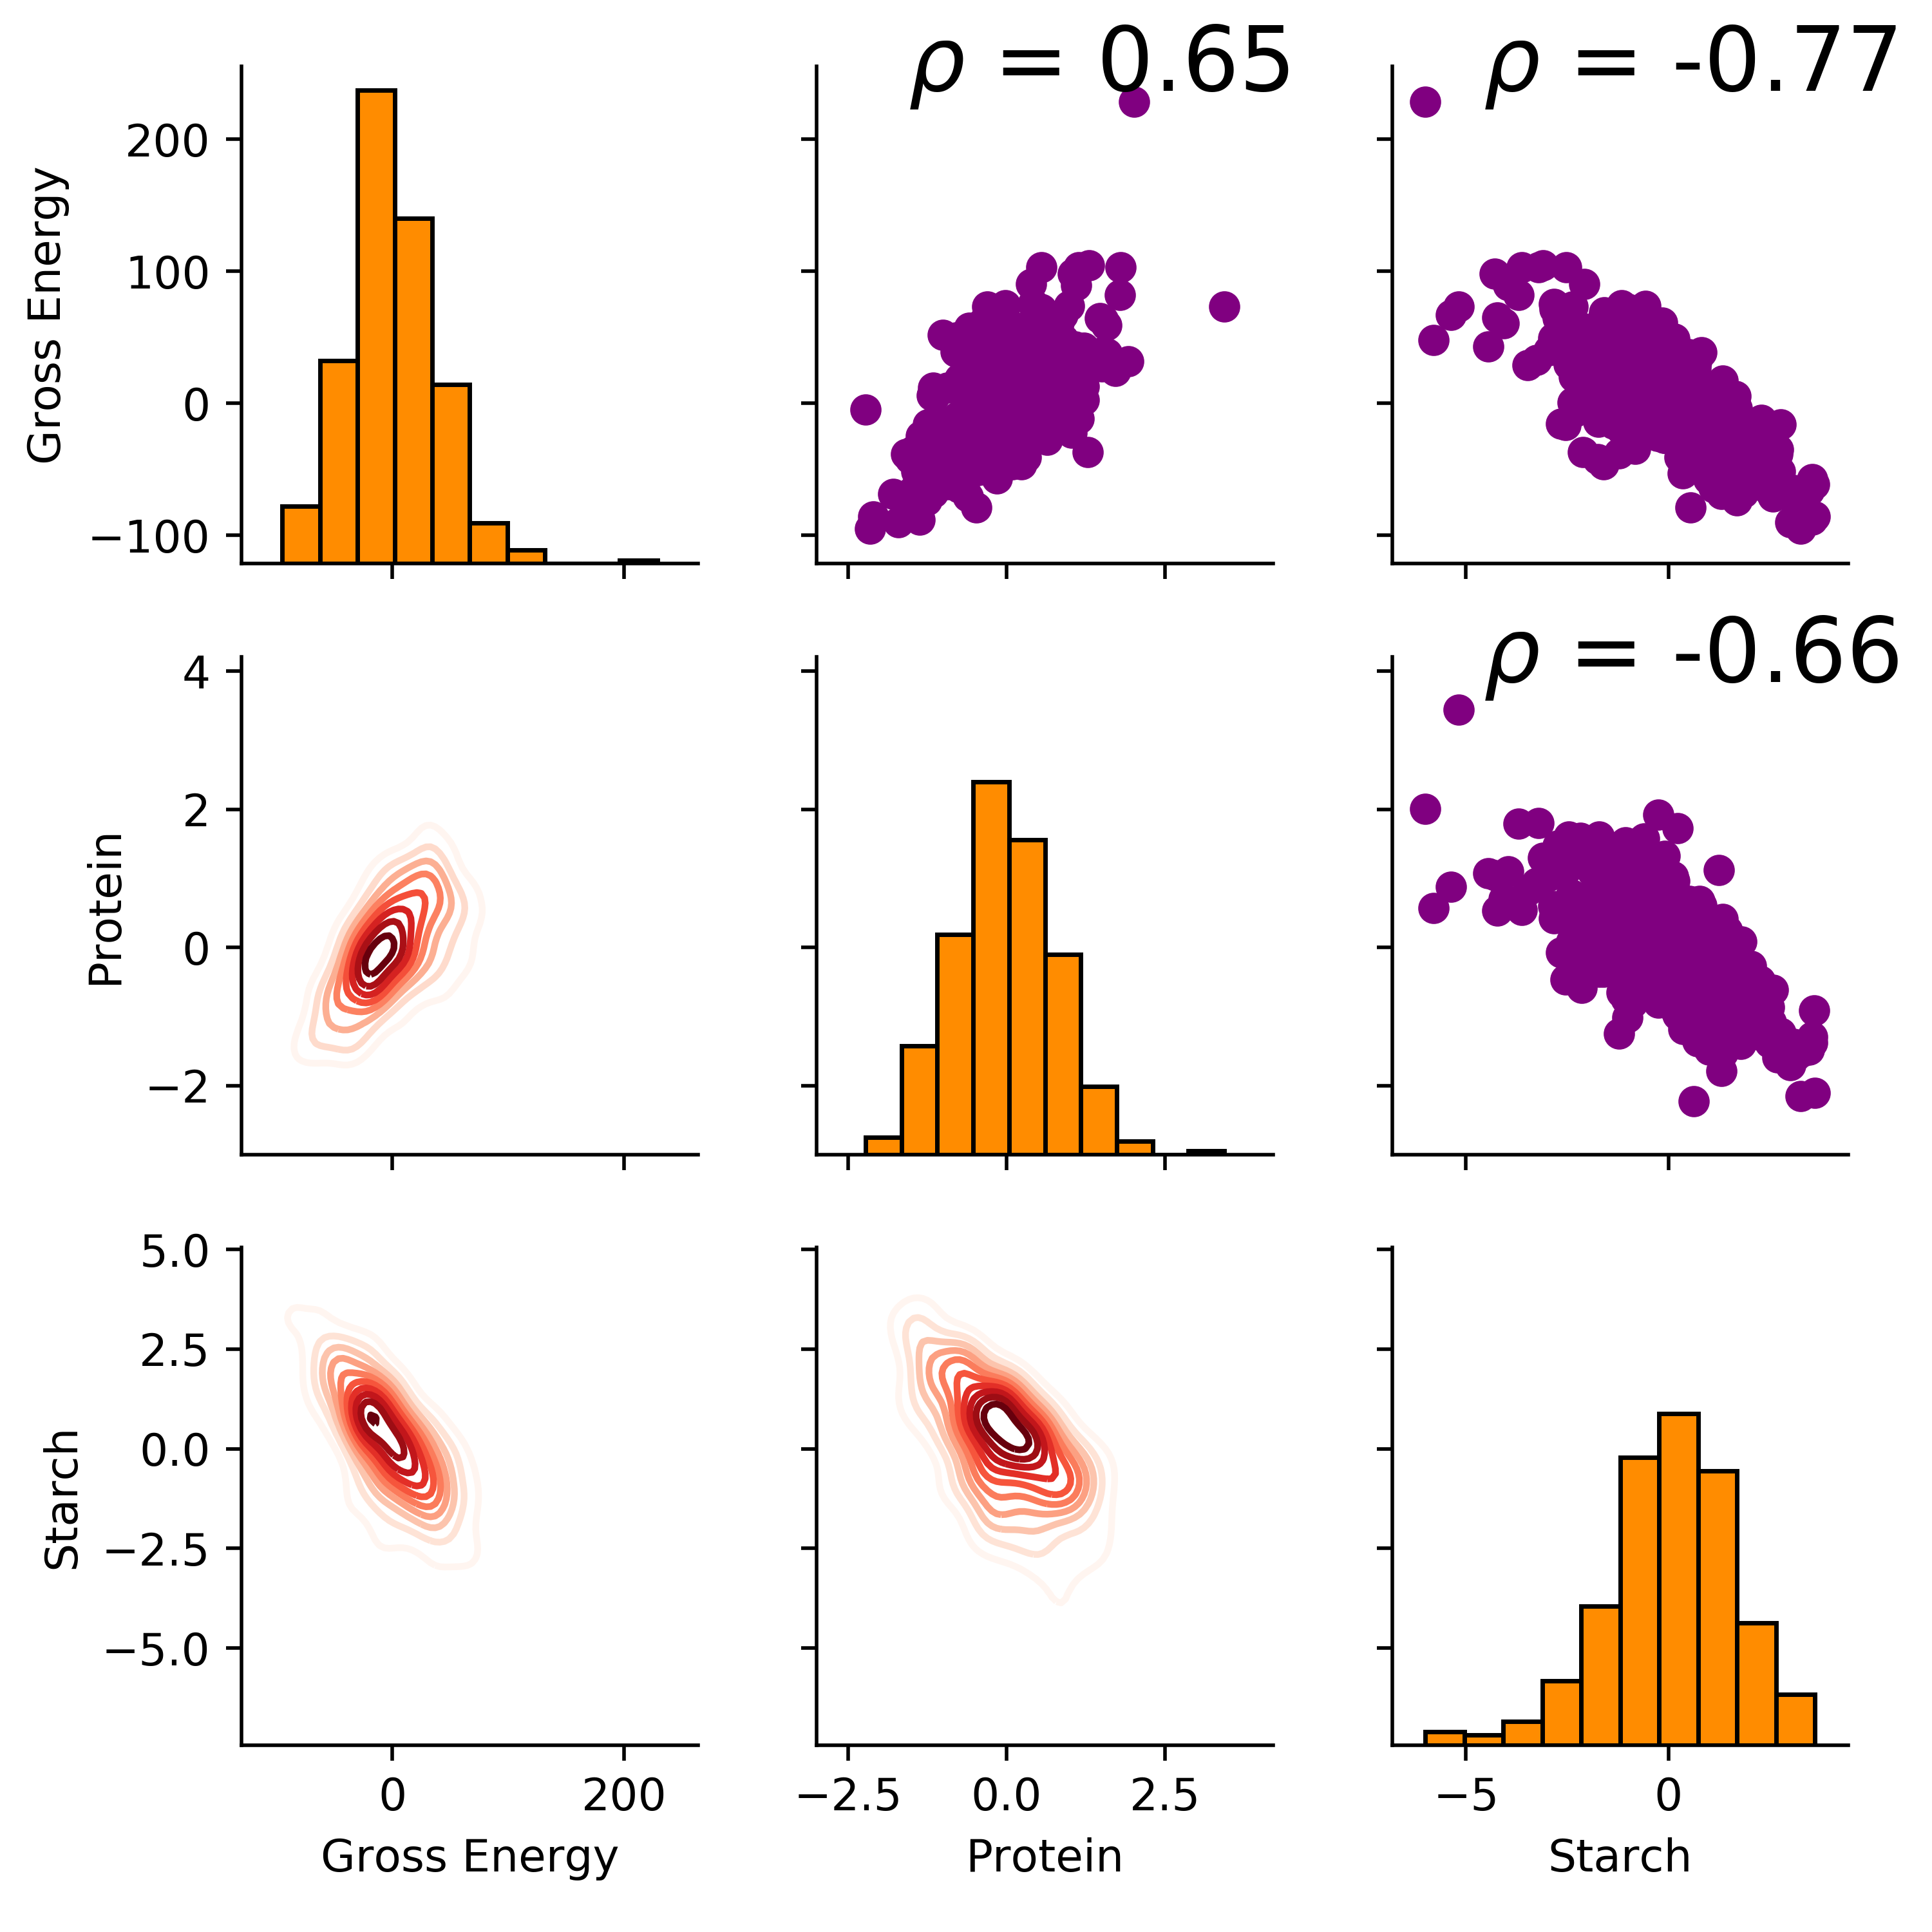
\includegraphics [height=55mm, width=55mm] {PairGrid_GSDP_SPG.png}
\end{center}
\small{\textbf{Figure 2.} Distribution and correlation of BLUPs.}
}
%----------------------------------------------------------------------------------------
%	SUMMARY
%----------------------------------------------------------------------------------------
\headerbox{Summary}{name=summary,span=2,column=1,row=1, below=genenetwork}{
{
\begin{itemize}
    \itemsep0em 
    \item Protein and gross energy were significantly positively correlated to each other, but were significantly negatively correlated to starch.
    \item Starch had higher predictive ability (\textit{r}=0.6) than protein (\textit{r}=0.45), but there were no significant differences in predictive ability between various prediction models.
    \item Use of multivariate (MV) mixed model for highly correlated starch and protein showed increased statistical power over univariate approach. Significant associations were identified in chromosomes 4 and 8 using the MV approach.
    \item Several metabolic pathways, including protein metabolism, were found enriched in a KEGG enrichment analysis using high confidence first interactors (0.7) of the genes within 20 kb of significant SNPs.
    \item The genes identified within the associated regions could be potential hub genes involved in key regulatory and functional pathways for sugar/starch metabolism and grain filling.
\end{itemize}}
}

%----------------------------------------------------------------------------------------
%	REFERENCES
%----------------------------------------------------------------------------------------
%\headerbox{References}{name=references,column=1,below=conclusion,span=2}{

%}
%----------------------------------------------------------------------------------------
%	ACKNOWLEDGEMENTS
%----------------------------------------------------------------------------------------
\headerbox{Acknowledgments}{name=acknowledgements,column=0,row=2,below=genopheno}
{
\begin{center}

\includegraphics [height=7mm, width=70mm] {funding_sources2.png}
\end{center}
}
\end{poster}
\end{document}